\chapter{Preliminaries}\label{sec:preliminaries}

\section{Motivation}\label{sec:motivation}

Brain–Computer Interfaces (\gls{BCI}) have emerged as a powerful class of technologies that enable direct communication between the brain and external devices. These systems are increasingly being applied in neurorehabilitation, education, and clinical diagnosis due to their ability to monitor and interpret neural activity in real time \cite{luo2022review}. \glspl{BCI} have the potential to revolutionize the way cognitive s tates are assessed and modulated by offering closed-loop interaction mechanisms that adapt to the user’s brain dynamics \cite{Lim2023,Lin2025}. Central to this capability is the choice of neuroimaging modality, which must meet strict criteria in temporal resolution, portability, and cost-effectiveness—especially in applications involving children or naturalistic settings \cite{li2025flexible}.

Several neuroimaging techniques have been explored for use in \gls{BCI} systems, each with distinct advantages and limitations. Functional Magnetic Resonance Imaging (\gls{fMRI}) offers high spatial resolution and whole-brain coverage, but its cost, immobility, and dependence on specialized facilities make it impractical for real-time interaction or integration with everyday environments \cite{Yang2025}. Magnetoencephalography (\gls{MEG}) provides excellent spatiotemporal resolution but is similarly constrained by high operational costs and the need for magnetically shielded rooms \cite{Peksa2023}. Functional Near-Infrared Spectroscopy (\gls{fNIRS}), a more portable option, measures cortical hemodynamic responses with moderate spatial resolution and tolerance to movement \cite{Doherty2023}. However, its low temporal resolution limits its ability to capture fast-changing neural dynamics, such as those required for attentional monitoring or neurofeedback \cite{chen2023fnirs}.

Electroencephalography (\gls{EEG}), by contrast, emerges as the most suitable modality for \gls{BCI} applications that demand real-time responsiveness, portability, and affordability \cite{niso2023wireless}. \gls{EEG} records the brain's electrical activity through non-invasive scalp electrodes, offering millisecond-level temporal resolution ideal for tracking rapid cognitive events like attention shifts or inhibitory control. While \gls{EEG}'s spatial resolution is lower compared to \gls{fMRI} or \gls{MEG}, advances in signal processing—such as quantitative electroencephalography (\gls{QEEG}), functional connectivity analysis, and source localization—have greatly enhanced its ability to extract meaningful neurophysiological markers \cite{Caiado2025,Yadav2023, Varbu2022}. This practical advantage is highlighted when comparing brain imaging modalities along the spectrum of portability and infrastructure requirements (see Figure \ref{fig:neuroimaging_comparison}). Moreover, \gls{EEG}'s lightweight hardware, low infrastructure requirements, and compatibility with embedded systems make it an ideal foundation for interactive, portable, and scalable \gls{BCI} solutions \cite{cai2025high}.

\begin{figure}[h]
    \centering
    \includegraphics[width=1\textwidth]{Cap_1/Figures/Neuroimage.pdf}
    \caption{Comparison of neuroimaging modalities by spatial resolution, temporal resolution, and cost. \gls{EEG} stands out for its affordability, portability, and millisecond-level responsiveness.}
    \label{fig:neuroimaging_comparison}
\end{figure}

Building upon these practical advantages, \gls{EEG}-based \gls{BCI} systems have been widely adopted across a diverse range of non-clinical domains (see Figure \ref{fig:BCI_aplications}). In human-computer interaction and entertainment, for instance, motor imagery paradigms allow users to control digital interfaces or external devices simply by visualizing specific physical movements \cite{gao2022improving}. Similarly, in the emerging field of neuromarketing, \gls{EEG} is utilized to gauge consumer engagement and emotional valence in real-time, providing objective neurophysiological metrics that bypass the biases of traditional behavioral self-reporting \cite{byrne2022systematic}. Furthermore, visual experiments leveraging steady-state visually evoked potentials (SSVEPs) and other event-related potentials demonstrate \gls{EEG}'s capacity to create robust communication pipelines and monitor spatial attention \cite{chen2022spectrally}. These broad applications highlight the versatility of \gls{EEG} in decoding cognitive and sensory processes in everyday environments, seamlessly paving the way for more specialized, targeted interventions \cite{tait2025mobi}.


One of the most compelling clinical applications of \gls{EEG}-based \gls{BCI} is in the assessment and intervention of neurodevelopmental disorders such as Attention Deficit Hyperactivity Disorder (\gls{ADHD}). \gls{ADHD} affects approximately 10\% of children in Colombia \cite{salari2023global,pineda2003prevalence} and is characterized by persistent symptoms of inattention, hyperactivity, and impulsivity that interfere with academic performance, social relationships, and emotional regulation. Conventional diagnostic practices rely heavily on behavioral questionnaires and clinical observation, which, while informative, are inherently subjective and susceptible to bias \cite{raiker2017accuracy}. In this context, \gls{EEG} offers a valuable alternative by enabling the objective measurement of neural correlates linked to attention and impulse control. Well-established \gls{EEG} biomarkers such as elevated theta/beta ratios and altered event-related potentials (e.g., P300) have been extensively validated in the \gls{ADHD} literature, making \gls{EEG} a scientifically robust and clinically relevant tool for real-time cognitive monitoring and neurofeedback interventions \cite{tan2025p300}.

\begin{figure}[h]
    \centering
    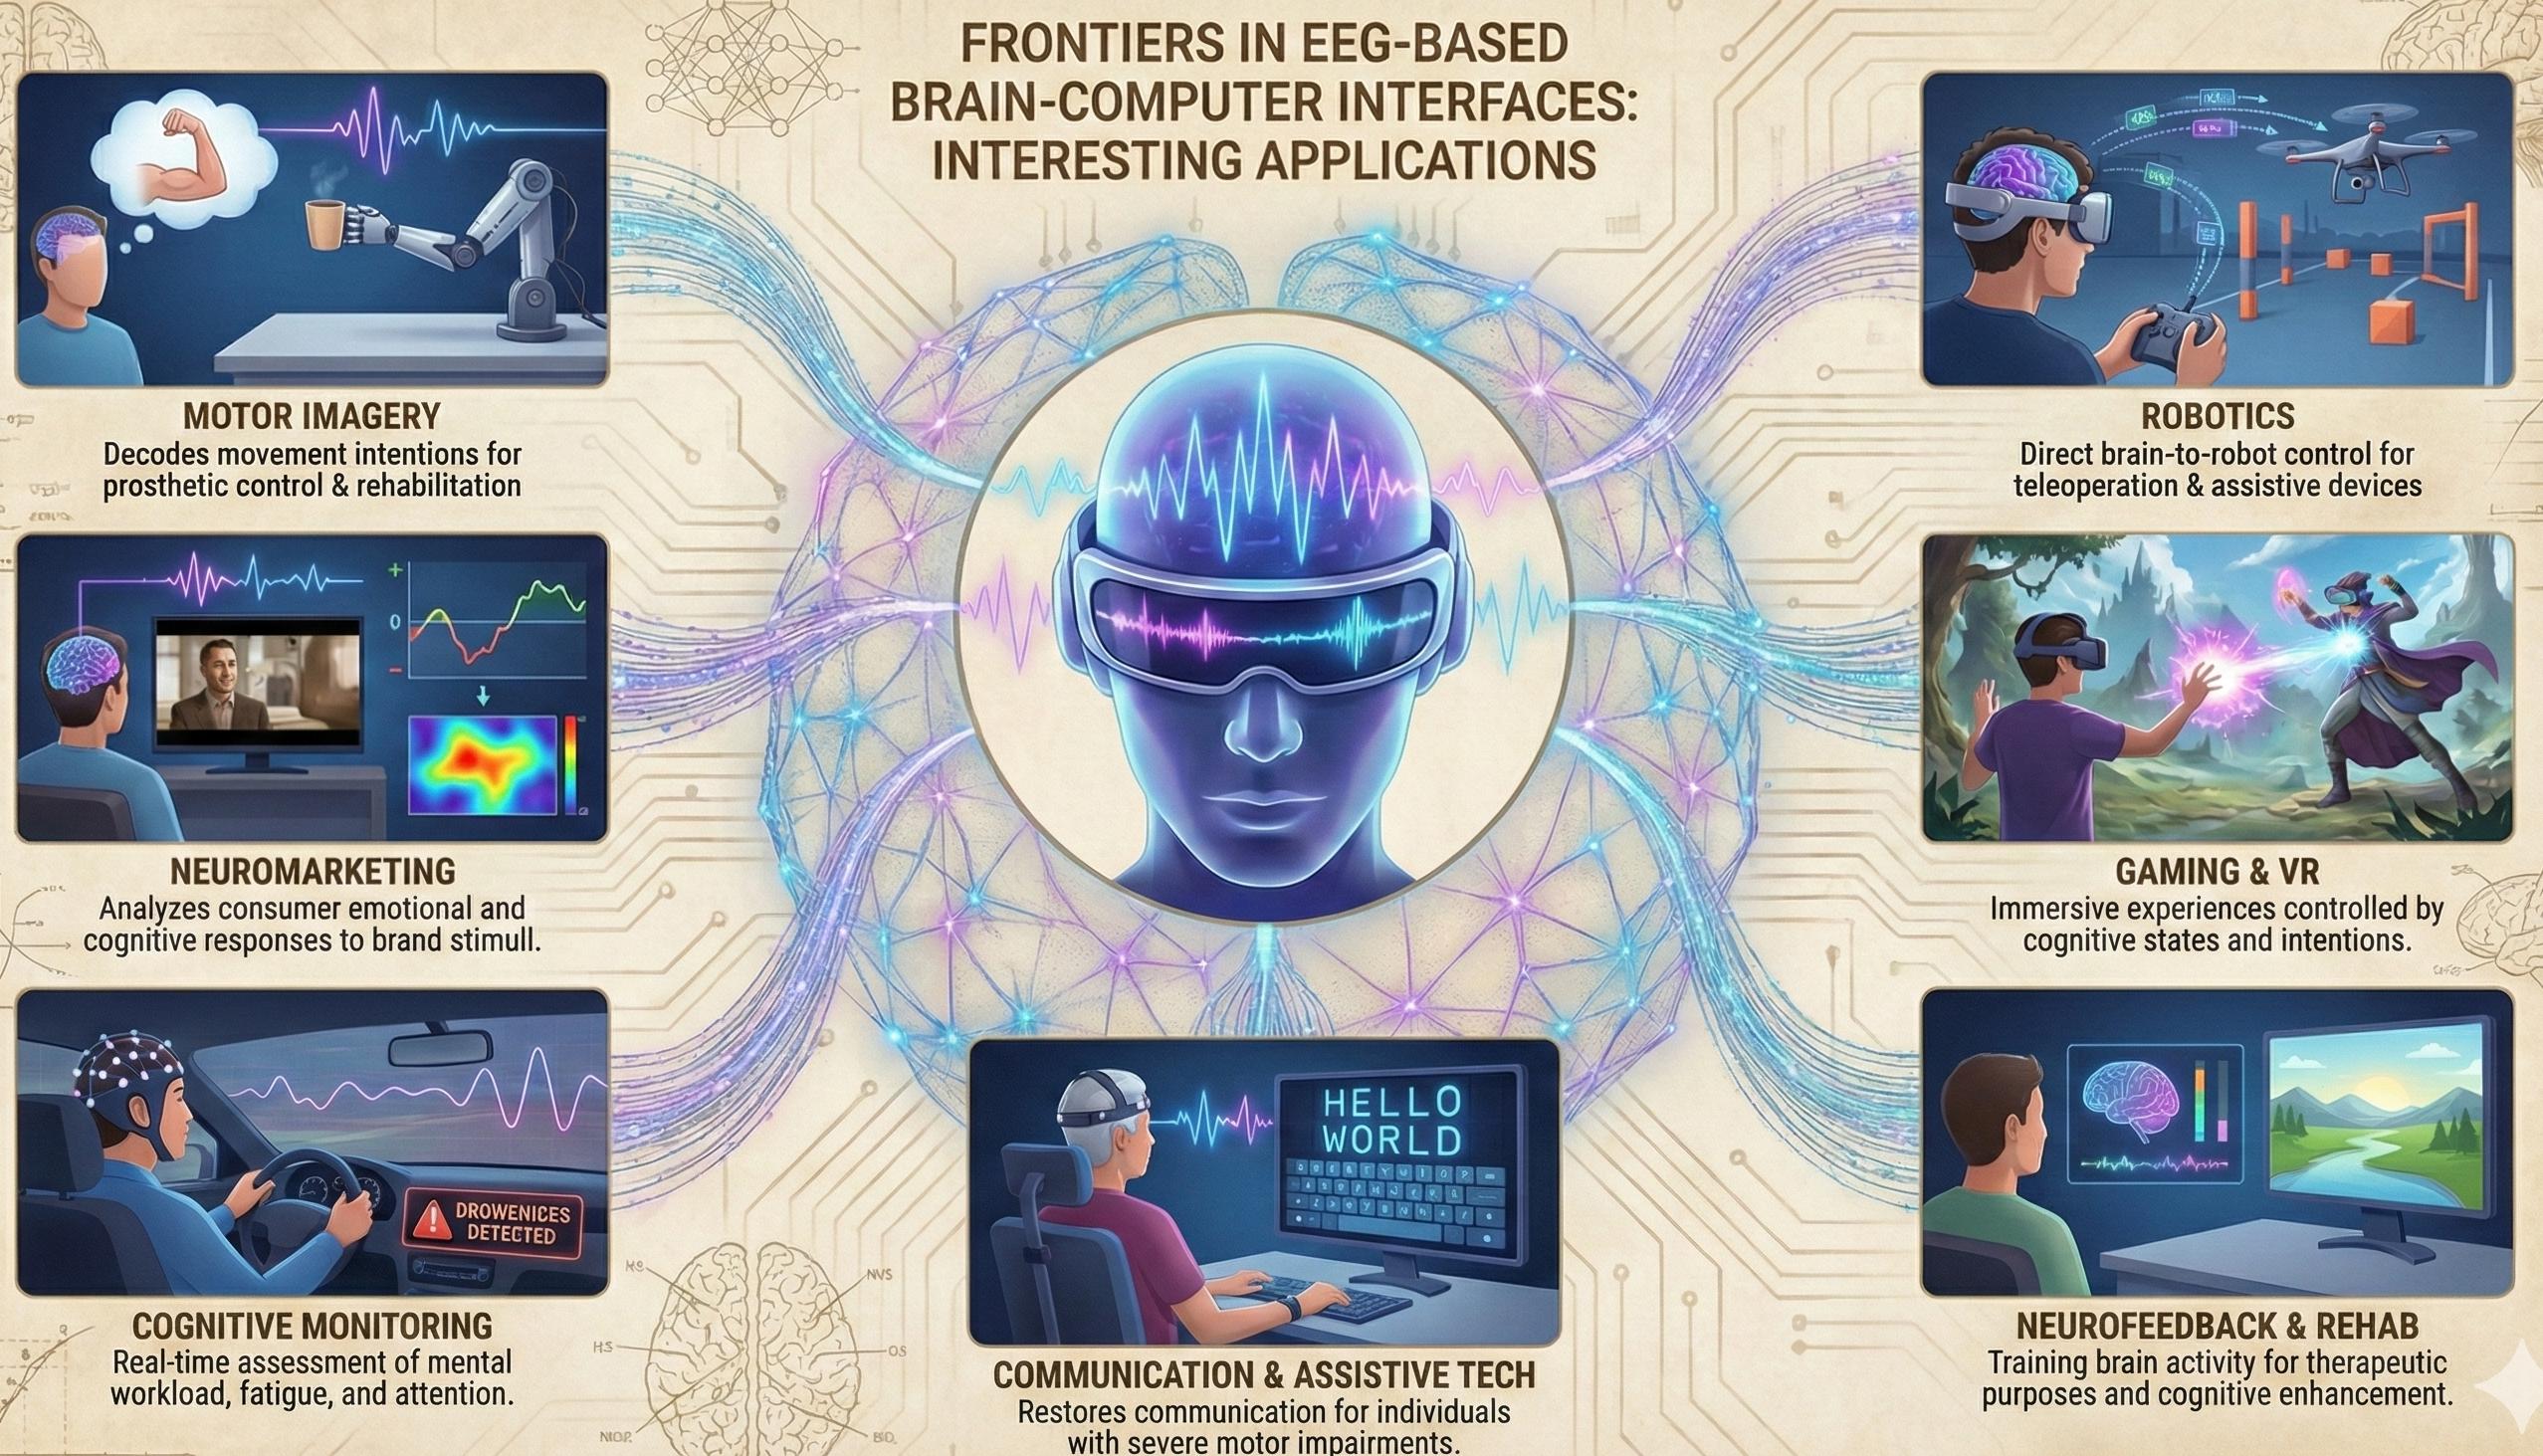
\includegraphics[width=1\textwidth]{Cap_1/Figures/Bci_apli2.png}
    \caption{Applications of EEG-based \glspl{BCI} in different domains.}
    \label{fig:BCI_aplications}
\end{figure}


Serious games are digital environments designed not solely for entertainment, but to fulfill educational, therapeutic, or cognitive objectives \cite{damavsevivcius2023serious}. In the context of neurodevelopmental disorders such as \gls{ADHD}, they have become increasingly relevant as tools for both cognitive assessment and intervention \cite{Patino2025}. Their engaging and adaptive nature allows them to target specific executive functions—like attention, inhibition, and working memory—while maintaining high user motivation, particularly among children \cite{RodriguezTimana2024}. To achieve this, two principal paradigms guide their design \cite{DeLuca2024}. The first is the task-based paradigm, which integrates classical neuropsychological tasks—such as the Go/No-Go, n-back, or Stroop test—into interactive game mechanics, allowing for the precise measurement of behavioral responses tied to well-established cognitive models \cite{Fang2025}. The second is the neurofeedback paradigm, in which the game dynamically responds to real-time EEG signals, offering auditory or visual feedback based on the user’s brain state. This paradigm supports operant conditioning mechanisms, encouraging users to self-regulate neural activity linked to attentional control and inhibition \cite{Firouzabadi2022}.

These design paradigms are intricately aligned with four core cognitive models critical to \gls{ADHD} pathology: attention, working memory, inhibition, and planning (see Figure \ref{fig:cognitive_models}). Games targeting the attentional model aim to improve sustained and selective attention, often requiring players to maintain focus amid distractions or shifting stimuli \cite{Chen2024}. Working memory is typically trained through tasks that require the temporary storage and manipulation of information, such as remembering sequences or updating mental representations. The inhibition model involves suppressing prepotent responses or resisting distractions—commonly implemented through fast-paced decision-making challenges or impulse control mechanics \cite{Takahashi2024, BreitlingZiegler2020}. Finally, the planning model emphasizes goal-directed behavior, encouraging users to sequence actions, solve multi-step problems, or anticipate future outcomes \cite{Lorini2022}. By aligning game mechanics with these cognitive models, serious games become powerful tools not only for engagement but for targeted neurocognitive intervention.

\begin{figure}[h]
    \centering
    \includegraphics[width=1\textwidth]{Cap_1/Figures/cognitive.pdf}
    \caption{Core cognitive models targeted by serious games in ADHD interventions: attention, working memory, inhibition, and planning. Each model maps to a specific set of game dynamics and EEG markers.}
    \label{fig:cognitive_models}
\end{figure}


When these targeted interventions are integrated with \gls{BCI} technology, they demonstrate substantial therapeutic benefits by reinforcing executive function, improving behavioral outcomes, and reducing symptom severity through active attention training \cite{Doulou2025}. By utilizing active \glspl{BCI}, in which users intentionally modulate their focus to influence the outcome of the game, these systems have been shown to strengthen cognitive control and promote long-term neuroplastic changes directly relevant to \gls{ADHD} pathology \cite{Cervantes2023}. Furthermore, these integrated platforms enable adaptive feedback, allowing interventions to dynamically adjust to each child's specific neurocognitive profile. Ultimately, combining robust cognitive models with real-time, objective EEG feedback makes serious games uniquely compatible with \glspl{BCI}, providing a highly personalized framework for interactive cognitive modulation.


Recent developments in portable EEG hardware have expanded the applicability of \glspl{BCI} for \gls{ADHD} beyond clinical settings, enabling real-time monitoring and feedback in homes, classrooms, and therapeutic environments (see Figure~\ref{fig:system_overview}). Low-cost, wireless EEG headsets—equipped with dry electrodes and embedded microcontrollers—have been successfully integrated into neurofeedback systems and serious games designed for children \cite{Xu2018}. These platforms allow for real-time signal acquisition and onboard processing, supporting closed-loop interventions without reliance on external computers. Thanks to ARM-based processors and system-on-chip (SoC) designs, it is now possible to run lightweight machine learning models directly on the device for real-time EEG classification \cite{Wang_2020}. Moreover, custom head-mounted EEG systems have shown reliable tracking of the theta/beta ratio, a key biomarker for \gls{ADHD}, during interactive tasks \cite{Larocco2020}.

\begin{figure}[h]
    \centering
    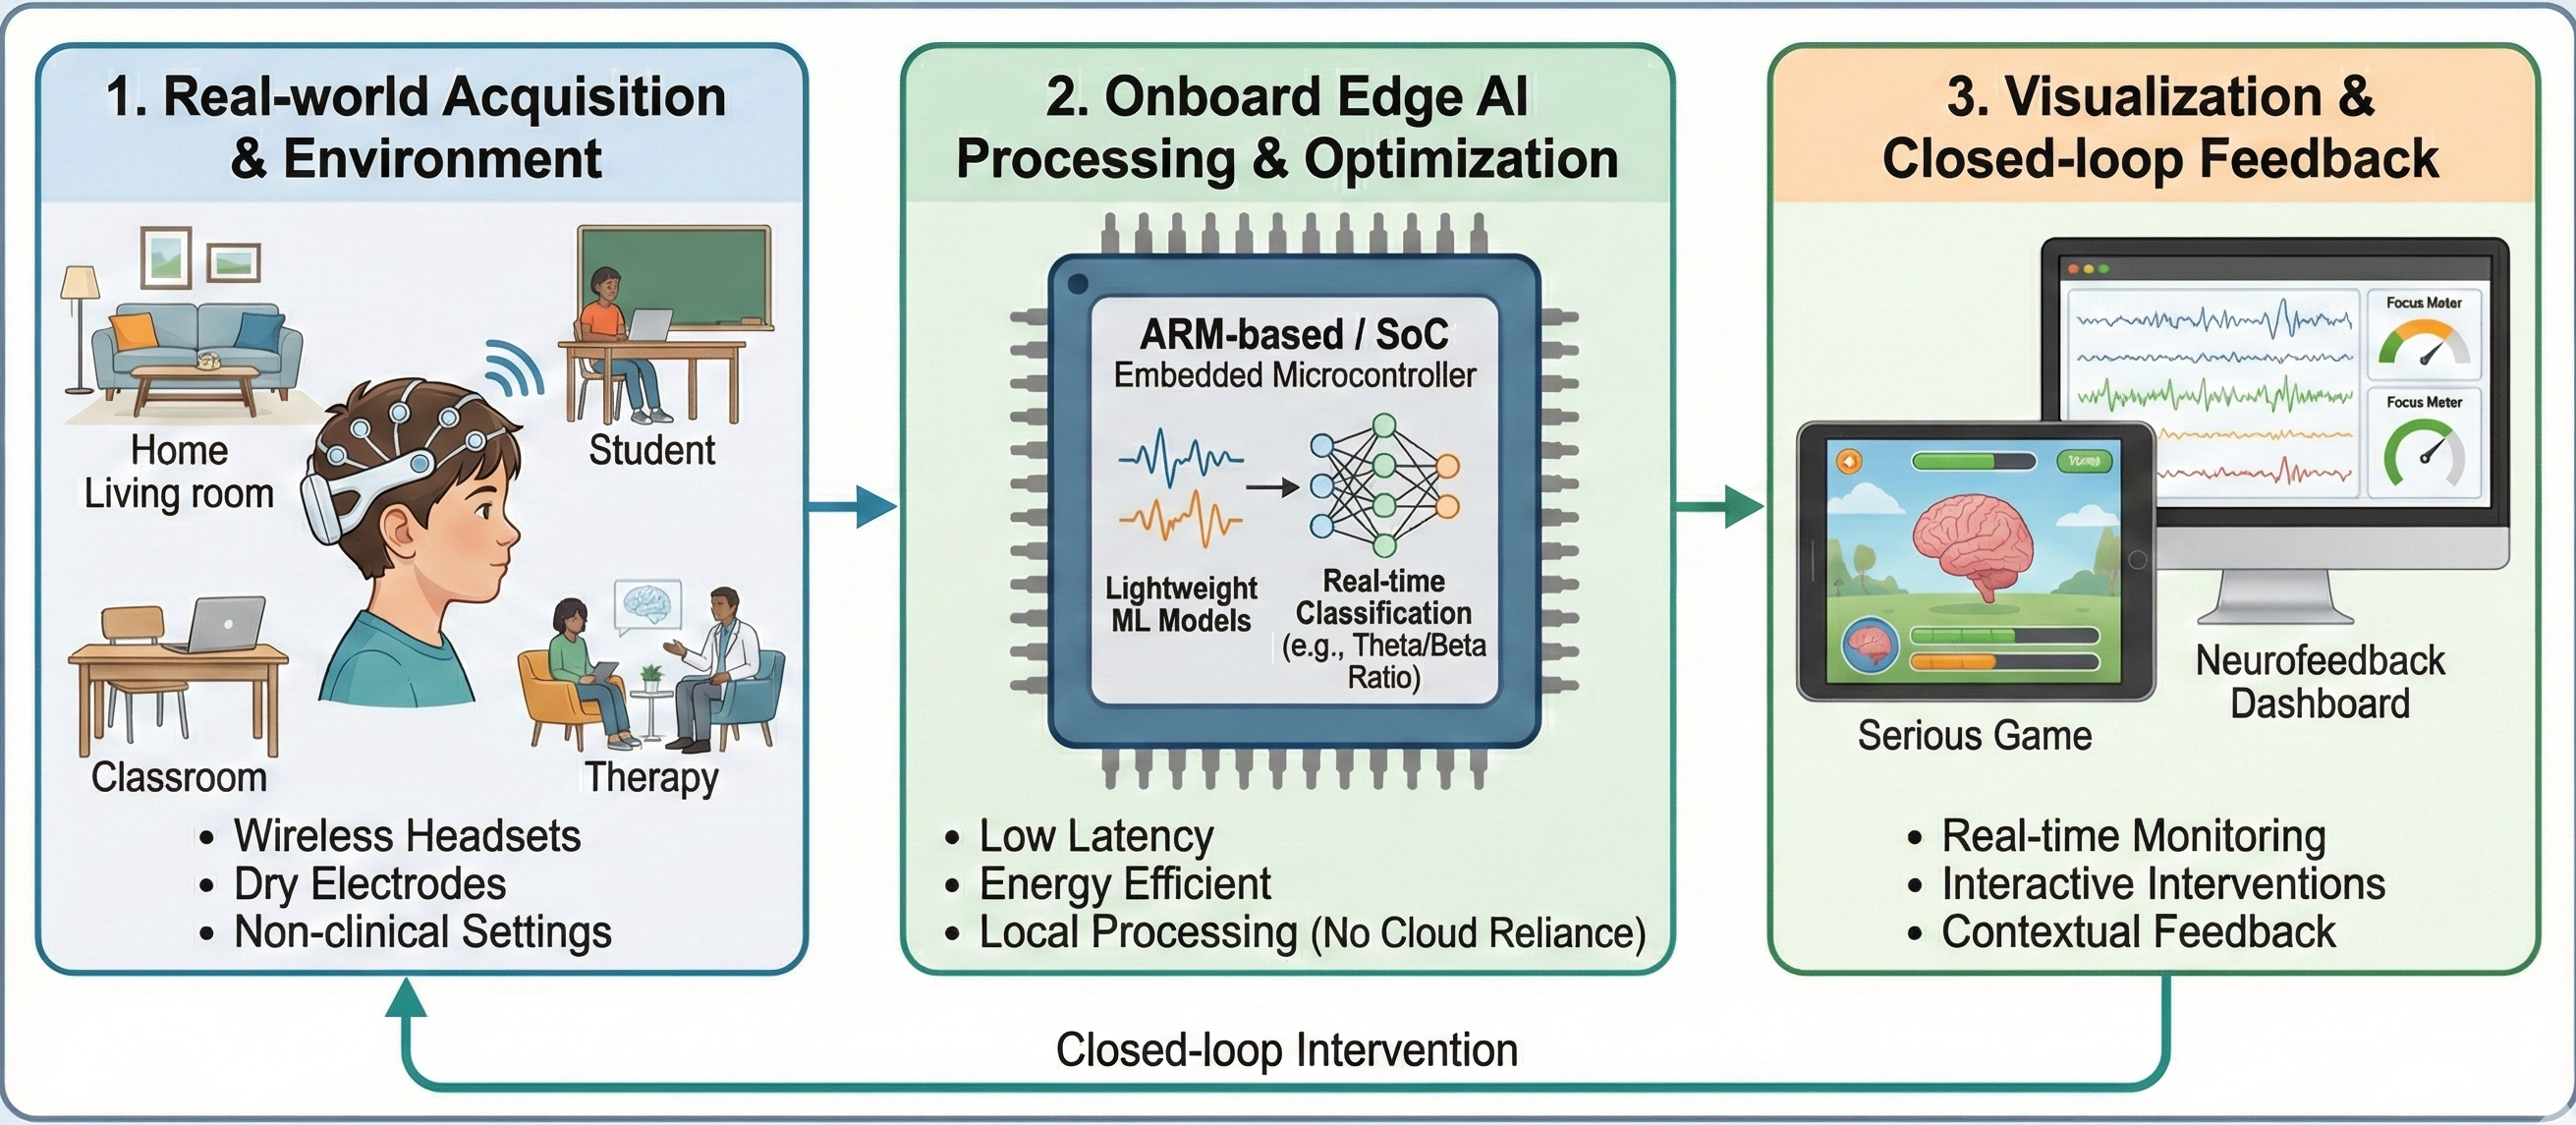
\includegraphics[width=1\textwidth]{Cap_1/Figures/BCI_IA.png}
    \caption{Overview of the Brain-Computer Interface (BCI) and Artificial Intelligence (AI) integration for neurocognitive assessment.}
    \label{fig:system_overview}
\end{figure}

The push to bring these portable, AI-driven interventions out of the clinic is heavily supported by the rapid expansion of the digital health sector. As of 2024, the global telehealth and telemedicine market surpassed \$123 billion, reflecting a permanent shift toward decentralized care and remote patient monitoring \cite{grandview_telehealth_2024}. To support this transition, the global embedded systems market reached over \$112 billion in 2024, driven by an immense demand for compact, energy-efficient Internet of Medical Things (IoMT) devices \cite{coherent_embedded_2024}. Concurrently, the integration of artificial intelligence into healthcare—a market valued at over \$13 billion in the U.S. alone in 2024—demonstrates a strong clinical and commercial drive to embed complex diagnostic intelligence directly into everyday environments \cite{novaone_ai_healthcare_2024}. These economic indicators highlight a clear motivation: there is a profound necessity to translate hospital-grade capabilities into accessible, wearable form factors that operate autonomously.

To successfully deploy these autonomous systems in daily life, research must focus on optimizing hardware and software integration for strict portable constraints \cite{phiri2023adaptive}. Operating continuously in non-clinical settings necessitates highly efficient energy and resource use, as wearable devices are bound by severe power and memory limitations. Processing biosignals locally via edge AI reduces latency and power-heavy cloud transmissions, yet it requires highly tailored acquisition algorithms that maximize computational efficiency \cite{shajari2023emergence}. Furthermore, capturing a comprehensive physiological profile demands the precise synchronization of biomarkers across distributed sensors \cite{ramasubramanya2025wearable}. Ensuring that multi-modal data streams are temporally aligned is an absolute necessity for generating accurate, real-time contextual feedback. By establishing robust methods to efficiently acquire, align, and process these integrated biomarkers on low-power architectures, this research aims to unlock the full therapeutic potential of continuous, closed-loop neurofeedback outside of traditional medical facilities \cite{li2023application}.



To address these evolving requirements for decentralized mental health technology, this research is developed within the framework of the project called ``Alianza científica con enfoque comunitario para mitigar brechas de atención y manejo de trastornos mentales relacionados con impulsividad en Colombia'' (\gls{ACEMATE}) (Multimodal system supported by serious games for personalized neurocognitive assessment and intervention in impulsivity disorders associated with ADHD), a collaborative initiative involving the Universidad Nacional de Colombia and the Universidad Tecnológica de Pereira. \gls{ACEMATE} aims to facilitate both face-to-face and remote interventions across clinical, educational, and community settings. However, realizing this vision of accessible care relies entirely on deploying physical infrastructure that resolves the previously outlined technical bottlenecks—specifically, the need for robust, portable hardware capable of precise biomarker synchronization. Consequently, this thesis proposes the development of MONEEE, a specialized EEG signal acquisition system designed to serve as the hardware enabler for \gls{ACEMATE}. By ensuring low-latency marker integration and high signal fidelity under strict energy and resource constraints, MONEEE provides the essential technological foundation to power the broader \gls{ACEMATE} ecosystem, ultimately democratizing access to objective, technology-driven mental health services for children.

\begin{figure}[h]
    \centering
    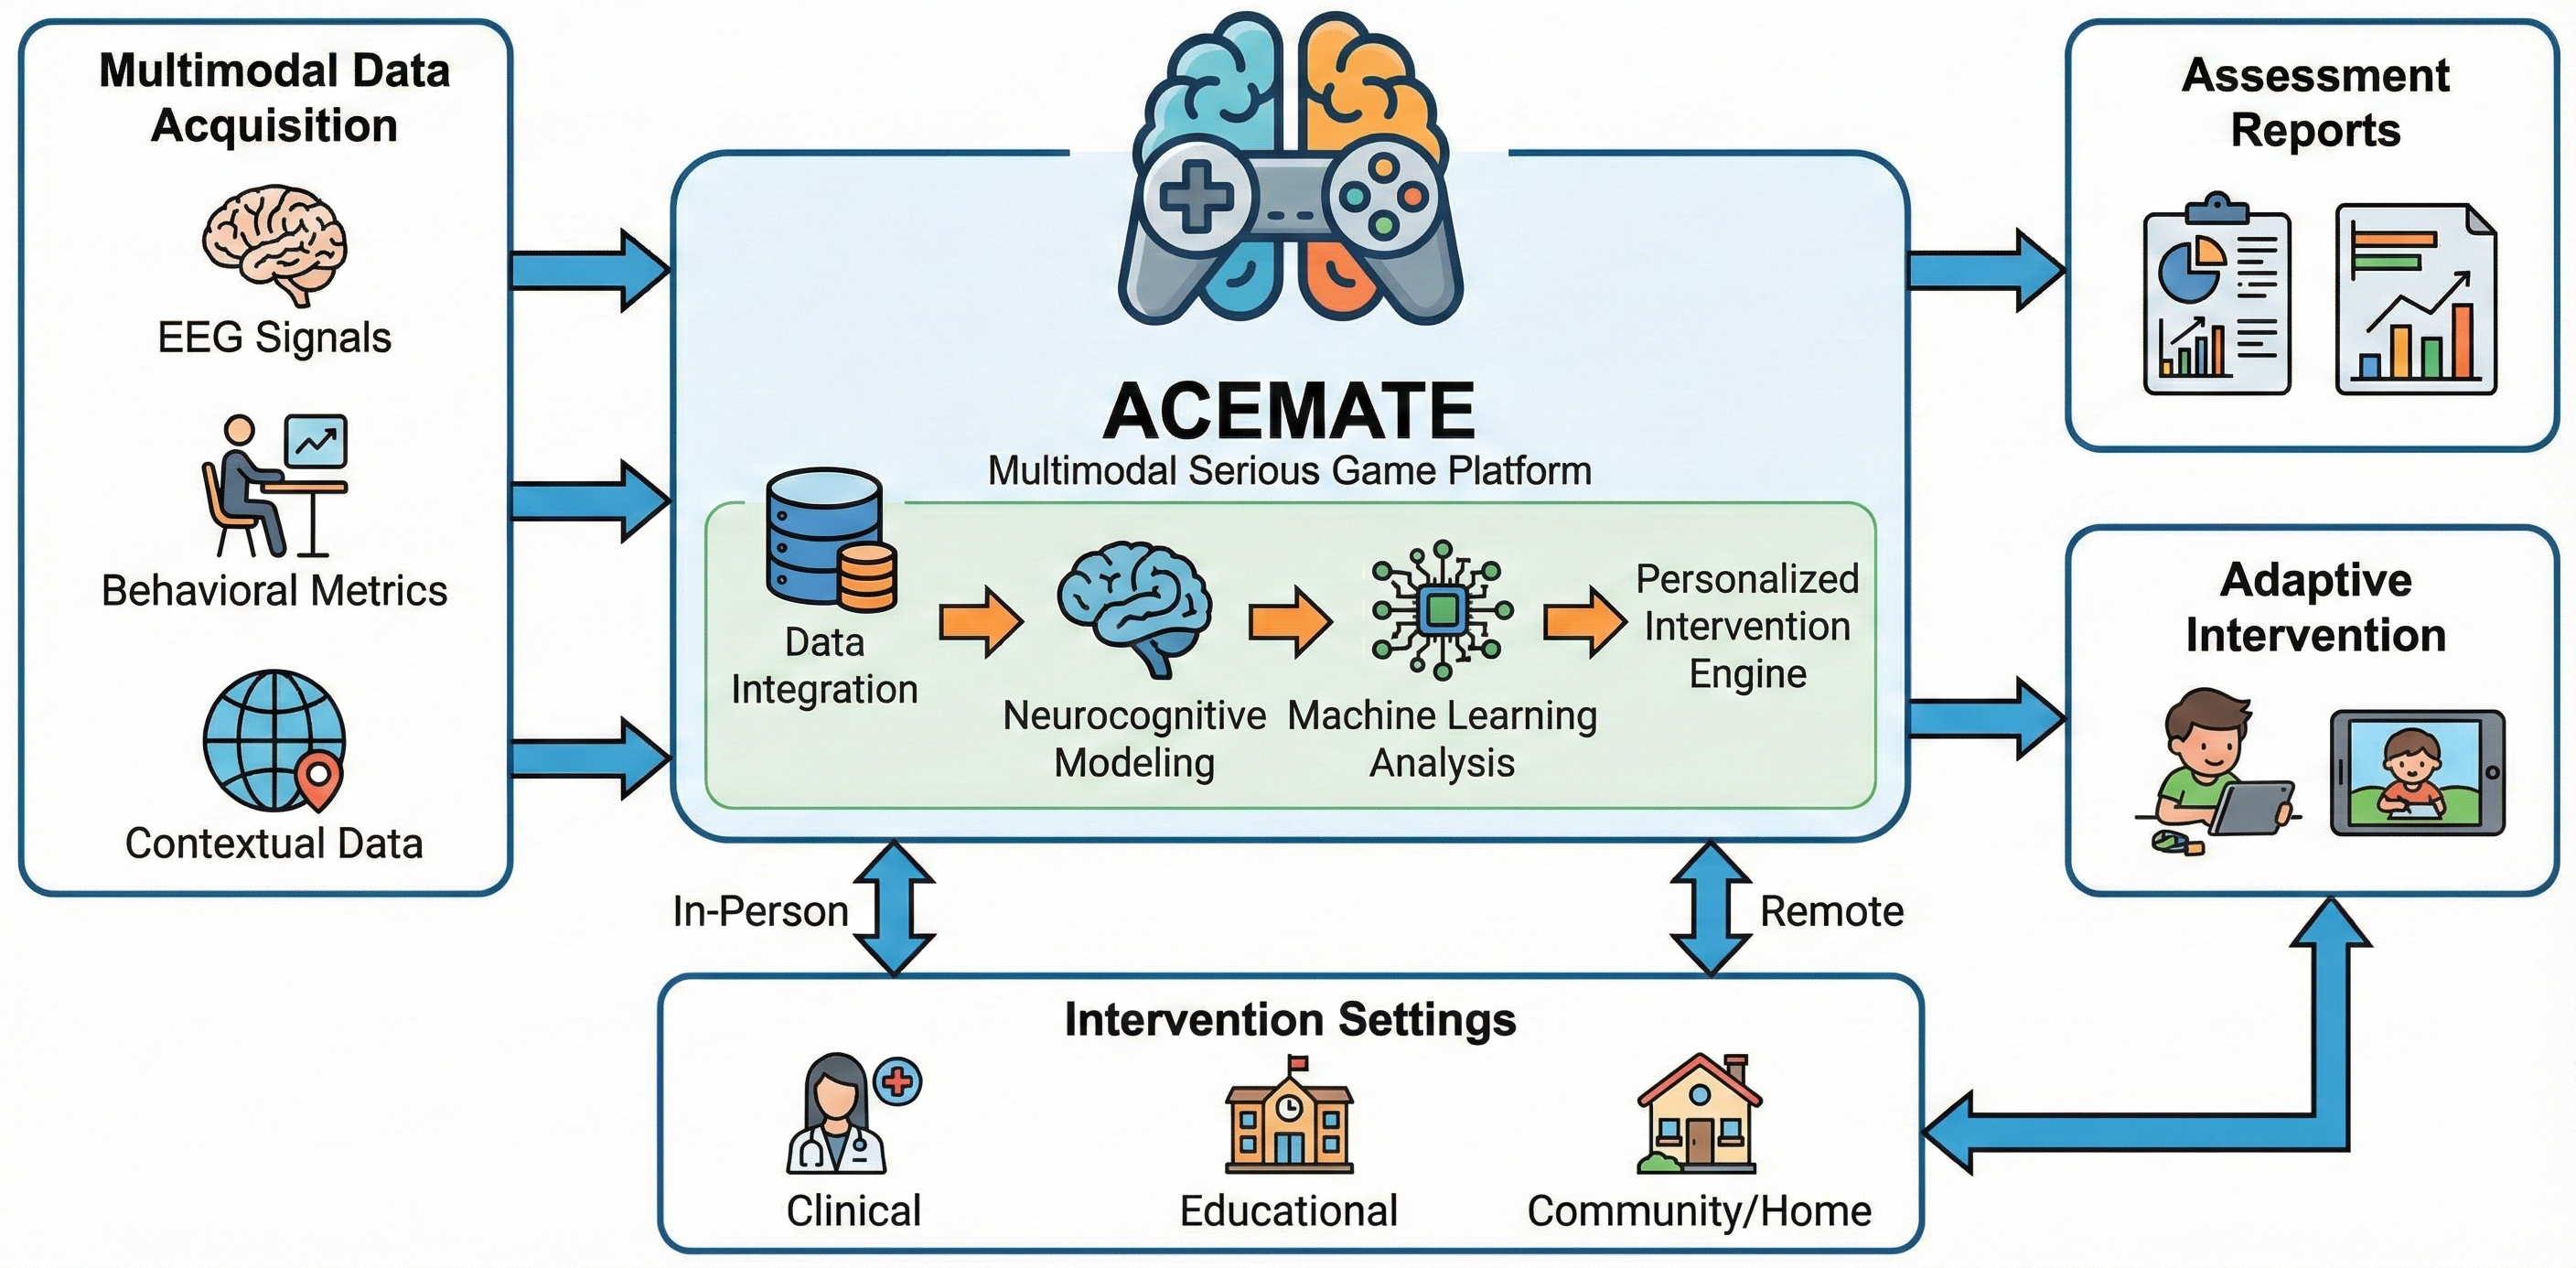
\includegraphics[width=1\textwidth]{Cap_1/Figures/acemate.png}
    \caption{Overview of the \gls{ACEMATE} project.}
    \label{fig:acemate}
\end{figure}


